\documentclass[12pt]{article}
\usepackage{tikz, rotating}
\usepackage{multirow}
\usepackage[active, tightpage]{preview}
\PreviewEnvironment{tikzpicture}
\setlength\PreviewBorder{0pt}

\begin{document}
\begin{tikzpicture}
  \node[draw, text width=1.5cm] (a) at (-6cm, 0) {Crawler};
  \node[draw, text width=1.6cm] (b) at (-3cm, 0) {Shot \\ Detector};
  \node[draw, text width=2.3cm] (c) at (1cm, 0) {Approximate Nearest Neighbor Lookup};
  \node[draw, text width=1.8cm] (d) at (5cm, 0) {Frequent Item Set Mining};
  \node[draw, text width=2cm] (e) at (8.5cm, 0) {Subsequent Mining};
  \node[text width=2cm] (f) at (12.5cm, 0) {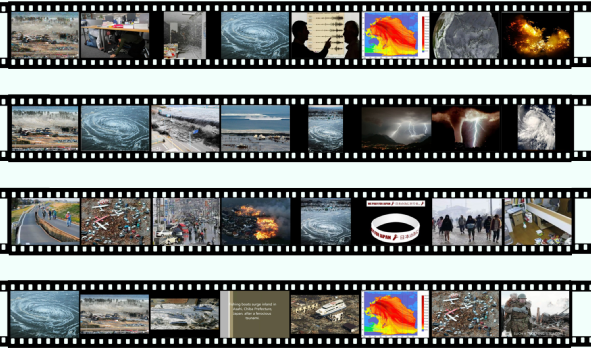
\includegraphics[scale=.1]{./img/sequence.png}};

  \draw[->] (a) -- node[above]{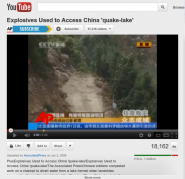
\includegraphics[scale=.1]{./img/video.png}} node[below]{\small $video$} (b);
  \draw[->] (b) -- node[above]{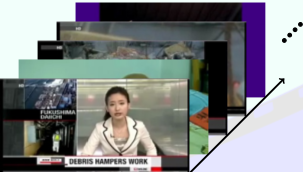
\includegraphics[scale=.1]{./img/shot.png}} node[below]{\small $shot$} (c);
  \draw[->] (c) -- node[above]{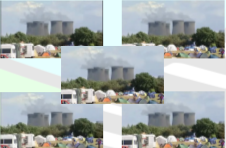
\includegraphics[scale=.1]{./img/duplicate.png}} node[below, text width=1cm]{\small $visual$ \\ $meme$} (d);
  \draw[->] (d) -- node[below]{$FIS$} (e);
  \draw[->] (e) -- node[below]{sequence} (f);
\end{tikzpicture}
\end{document}

%%% Local Variables: 
%%% mode: latex
%%% TeX-master: t
%%% End: 

%%% Local Variables:
%%% mode: latex
%%% TeX-master: t
%%% End:
